\documentclass{article} % For LaTeX2e
\usepackage{nips12submit_e,times}
\usepackage{amsmath}
\usepackage{graphicx}
\usepackage{caption}
\usepackage{subcaption}
\usepackage[top=1.0in, bottom=1.0in, left=1.0in, right=1.0in]{geometry}

%\renewcommand\refname{Papers To Read}
\title{Semantic Segmentation Using Hybrid Markov Logic Networks}

\author{
Aravindh Mahendran \\
\texttt{amahend1@andrew.cmu.edu} \\ 
\And
Nitish Thatte \\
\texttt{nitisht@andrew.cmu.edu} \\
\AND
Adwait Gandhe \\
\texttt{agandhe@andrew.cmu.edu} \\
}

\newcommand{\fix}{\marginpar{FIX}}
\newcommand{\new}{\marginpar{NEW}}

\nipsfinalcopy

%------------------------------------------------------------------------------------------

\begin{document}
\maketitle

\begin{abstract}
In this paper, we propose a new approach for Semantic Segmentation using Hybrid Markov Logic Networks. 
\end{abstract}


\section{Introduction}


%------------------------------------------------------------------------------------------

\section{Related Work}

%------------------------------------------------------------------------------------------

\section{Method}

%------------------------------------------------------------------------------------------
\subsection{Label Propagation}
	In the related works section above, we discussed a method of propagating labels on a graph of connected superpixels based on a learned label transfer confidence function. This method introduced us to two ideas: propagating labels rather than directly minimizing a cost function to arrive at a segmentation and working with graphs of related superpixels. Building on these ideas, one approach we decided to pursue is to learn the weights for a hybrid Markov logic network in order to refine a prior expected segmentation obtained from a baseline algorithm through maximum a posteriori estimation. The method incorporates an undirected graph of connected superpixels that expresses where labels can propagate.

Examples of numeric terms and predicates in this Markov logic network are:

\begin{align*}
	&featureDistance(s_i,s_j)\\
	&isLabel(s_i,l_k) \\
	&isNeighbor(s_i,s_j)
\end{align*}

\noindent Where $s_i$ is the $i^\textrm{th}$ superpixel in an image and $l_k$ is the $k^\textrm{th}$ label. $featureDistance()$ is a numeric term that returns the computed distance between two image feature vectors via a distance metric such as euclidean or cosine distance. $isLabel()$ returns 1 if superpixel $s_i$ has label $l_j$ and 0 otherwise, and $isNeighbor$ returns 1 if its arguments are the neighbors and 0 otherwise. 

An example of a formula in this hybrid Markov logic network that use these predicates and numeric terms are :

\begin{equation*}
	[isNeighbor(s_i,s_j) \Rightarro (isLabel(s_i,l_k) \Leftrightarrow isLabel(s_k,l_m))]*(featureDistance(s_i, s_k, f_m))
\end{equation*}

\noindent This formula encodes the following two beliefs about how and why labels can propagate in the image.

\begin{enumerate}
\item
	Superpixels with similar feature vectors should have the same label.
\item
	Superpixels that are connected by an edge (are neighbors) should have the same label.
\end{enumerate}

A brute-force approach to this problem would be to allow every super pixel to transfer its label to every other superpixel. This would result in a complete graph, where there is an edge between every two distinct nodes. Such a graph would allow superpixel labels to be learned from a more global context in the image. However, there would be an immense number of formulas for which to learn weights, making finding the solution computationally intractable. 

In contrast, a simple approach, which has been attempted in the past, \cite{} %insert reference%
is to connect nodes that are directly share borders. Consequently, the graph would very few edges, greatly reducing the number of required learned weights and simplifying the learning problem. This approach, however, would only use local context for label propagation.

Therefore, we propose to take a middle ground approach that will produce densely connected superpixels where relations are expected to be strong, and fewer edges across boundaries expected to not share labels. In order build this superpixel graph, we take two levels of superpixel segmentations: A coarse level, which we will henceforth refer to as supersuperpixels, and a fine level, termed superpixels. All superpixels within a supersuperpixel are connected allowing for contextual information to be shared within a region. Additionally superpixels that share a boundary between two supersuperpixels are connected allowing for labels to propagate across supersuperpixels while acknowledging that label transfer across supersuperpixels is less probable than within a supersuperpixel.

\section{Experiment}

\begin{figure}
	\centering
	\begin{subfigure}[c]{\textwidth}
		\centering
		\begin{subfigure}[c]{0.195\textwidth}
			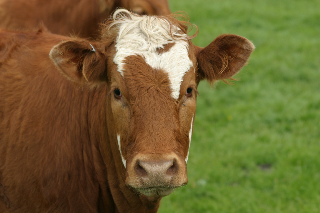
\includegraphics[width = \textwidth]{./img/1_22_s.png}
			\label{fig:1_22_s}
		\end{subfigure}
		\begin{subfigure}[c]{0.195\textwidth}
			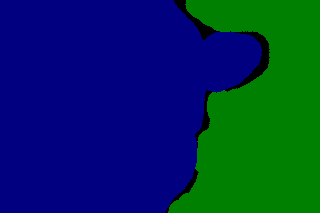
\includegraphics[width = \textwidth]{./img/1_22_s_GT.png}
			\label{fig:1_22_s_lab}
		\end{subfigure}
		\begin{subfigure}[c]{0.195\textwidth}
			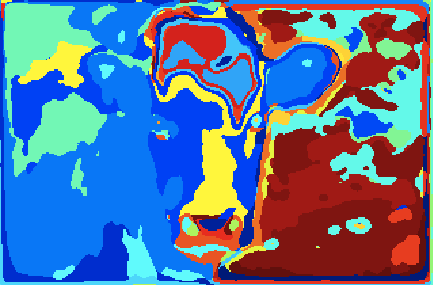
\includegraphics[width = \textwidth]{./img/1_22_s_map.png}
			\label{fig:1_22_s_map}
		\end{subfigure}
		\begin{subfigure}[]{0.195\textwidth}
			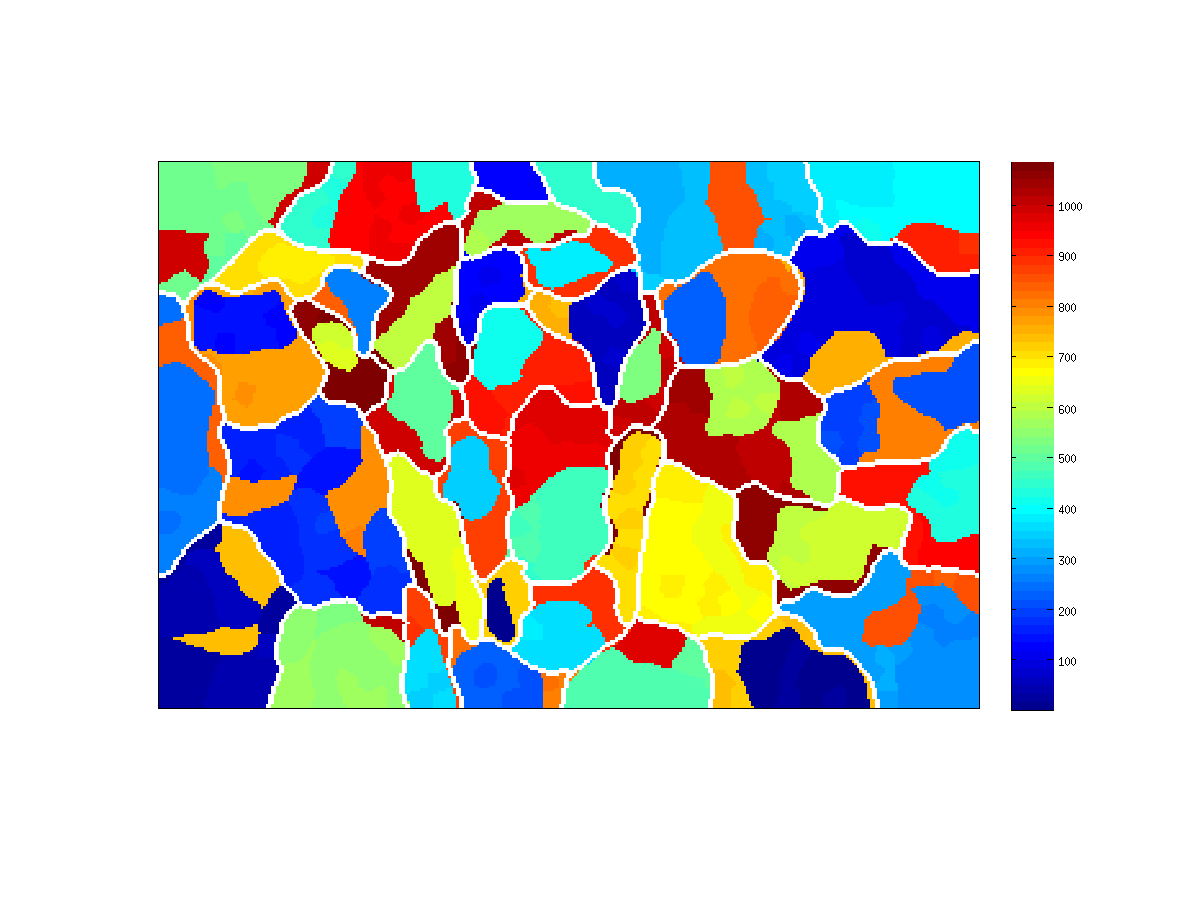
\includegraphics[width = \textwidth]{./img/su1_22_s.pdf}
			\label{fig:1_22_s_su}
		\end{subfigure}
		\begin{subfigure}[c]{0.195\textwidth}
			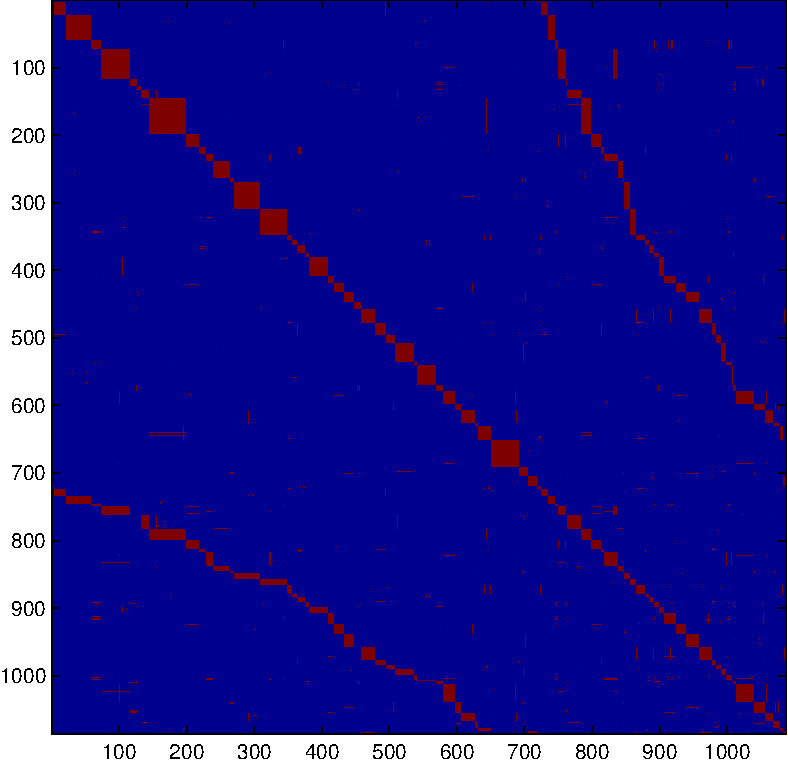
\includegraphics[width = \textwidth]{./img/adj1_22_s.pdf}
			\label{fig1_22_s_adj}
		\end{subfigure}
	\end{subfigure}

	\begin{subfigure}[c]{\textwidth}
		\centering
		\begin{subfigure}[c]{0.195\textwidth}
			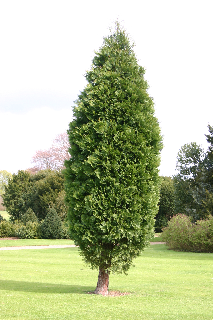
\includegraphics[width = \textwidth]{./img/2_21_s.png}
			\label{fig:2_21_s}
		\end{subfigure}
		\begin{subfigure}[c]{0.195\textwidth}
			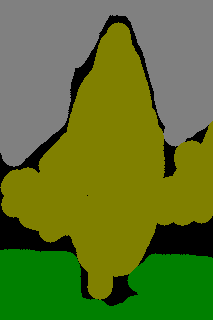
\includegraphics[width = \textwidth]{./img/2_21_s_GT.png}
			\label{fig:2_21_s_lab}
		\end{subfigure}
		\begin{subfigure}[c]{0.195\textwidth}
			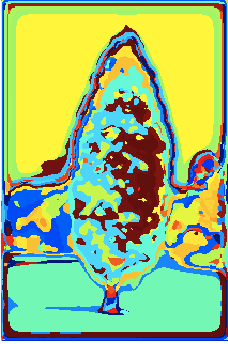
\includegraphics[width = \textwidth]{./img/2_21_s_map.png}
			\label{fig:2_21_s_map}
		\end{subfigure}
		\begin{subfigure}[]{0.195\textwidth}
			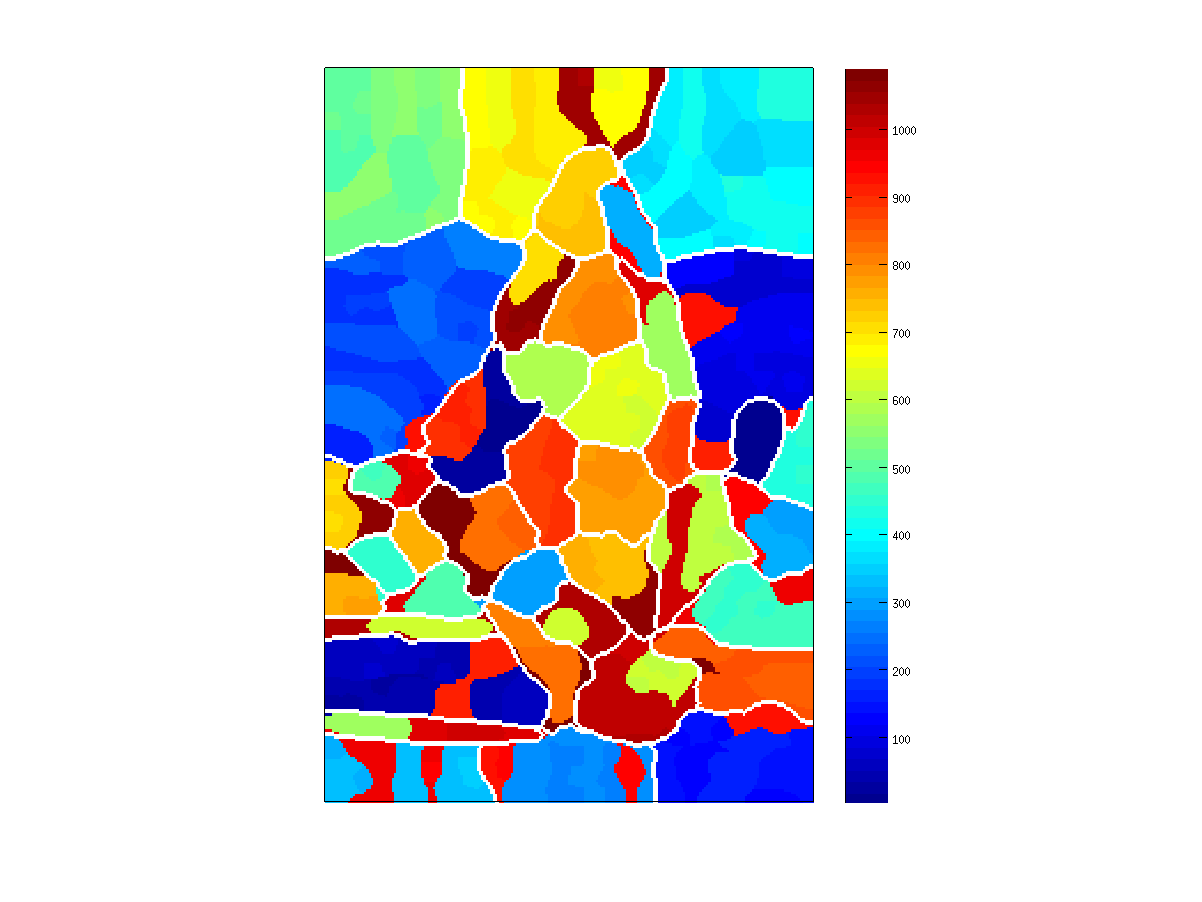
\includegraphics[width = \textwidth]{./img/su2_21_s.pdf}
			\label{fig:2_21_s_su}
		\end{subfigure}
		\begin{subfigure}[c]{0.195\textwidth}
			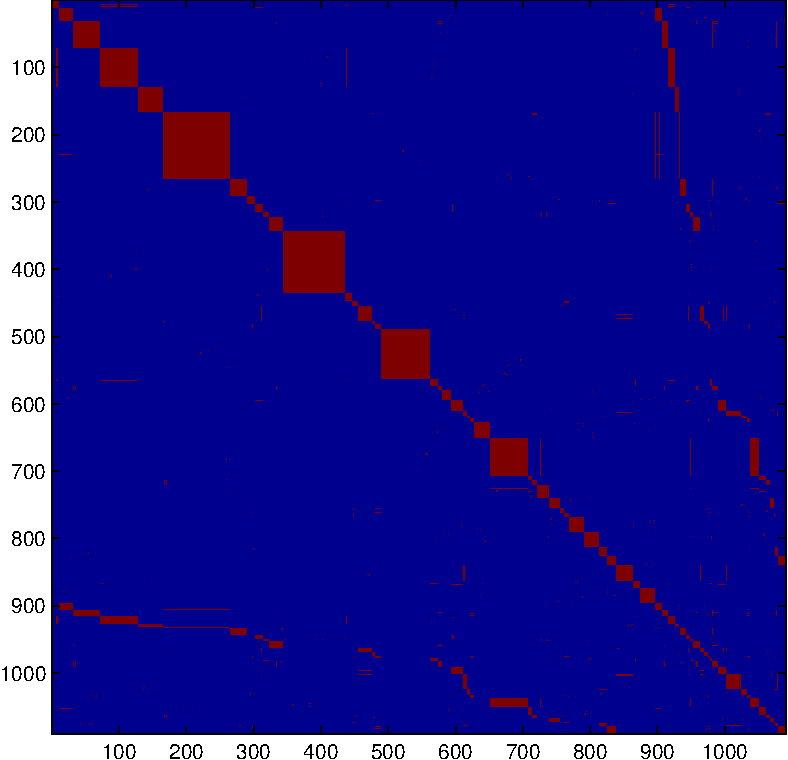
\includegraphics[width = \textwidth]{./img/adj2_21_s.pdf}
			\label{fig2_21_s_adj}
		\end{subfigure}
	\end{subfigure}

	\begin{subfigure}[c]{\textwidth}
		\centering
		\begin{subfigure}[c]{0.195\textwidth}
			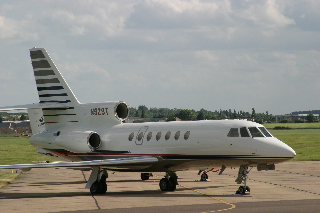
\includegraphics[width = \textwidth]{./img/4_1_s.png}
			\label{fig:4_1_s}
		\end{subfigure}
		\begin{subfigure}[c]{0.195\textwidth}
			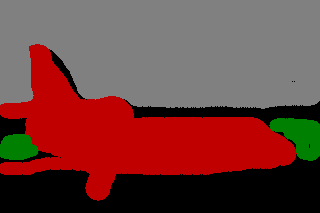
\includegraphics[width = \textwidth]{./img/4_1_s_GT.png}
			\label{fig:4_1_s_lab}
		\end{subfigure}
		\begin{subfigure}[c]{0.195\textwidth}
			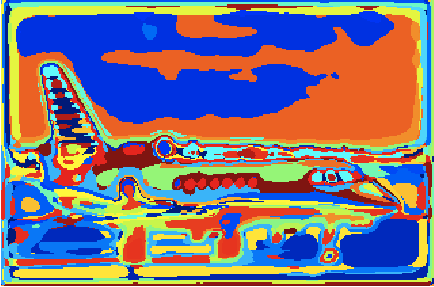
\includegraphics[width = \textwidth]{./img/4_1_s_map.png}
			\label{fig:4_1_s_map}
		\end{subfigure}
		\begin{subfigure}[]{0.195\textwidth}
			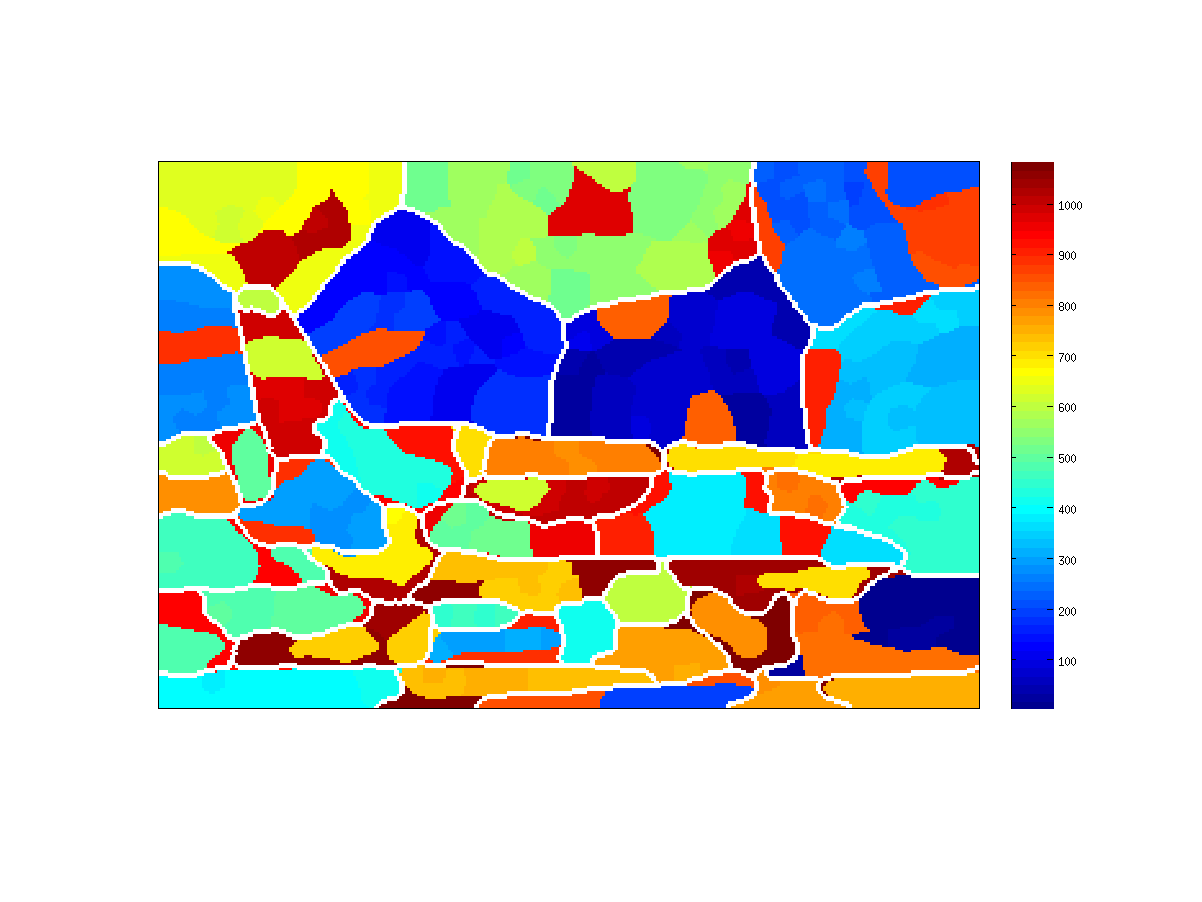
\includegraphics[width = \textwidth]{./img/su4_1_s.pdf}
			\label{fig:4_1_s_su}
		\end{subfigure}
		\begin{subfigure}[c]{0.195\textwidth}
			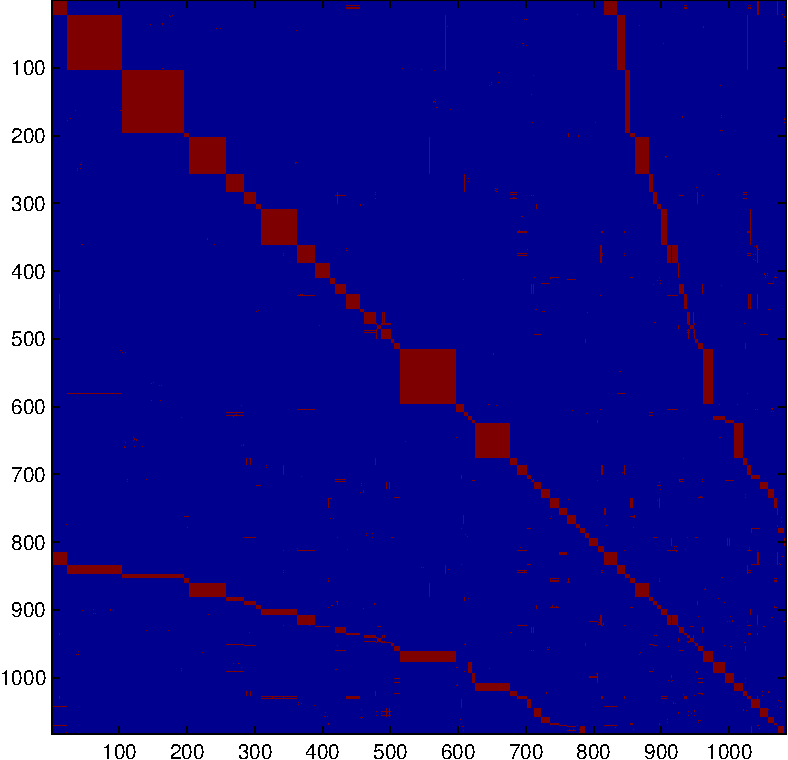
\includegraphics[width = \textwidth]{./img/adj4_1_s.pdf}
			\label{fig4_1_s_adj}
		\end{subfigure}
	\end{subfigure}

	\begin{subfigure}[c]{\textwidth}
		\centering
		\begin{subfigure}[c]{0.195\textwidth}
			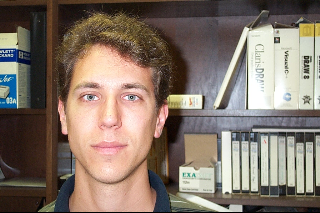
\includegraphics[width = \textwidth]{./img/6_3_s.png}
			\label{fig:6_3_s}
		\end{subfigure}
		\begin{subfigure}[c]{0.195\textwidth}
			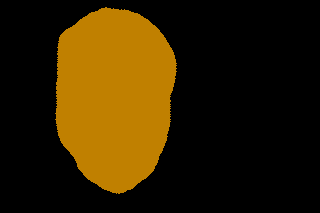
\includegraphics[width = \textwidth]{./img/6_3_s_GT.png}
			\label{fig:6_3_s_lab}
		\end{subfigure}
		\begin{subfigure}[c]{0.195\textwidth}
			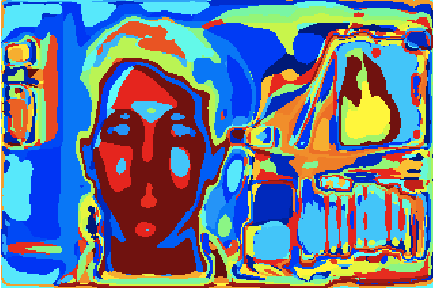
\includegraphics[width = \textwidth]{./img/6_3_s_map.png}
			\label{fig:6_3_s_map}
		\end{subfigure}
		\begin{subfigure}[]{0.195\textwidth}
			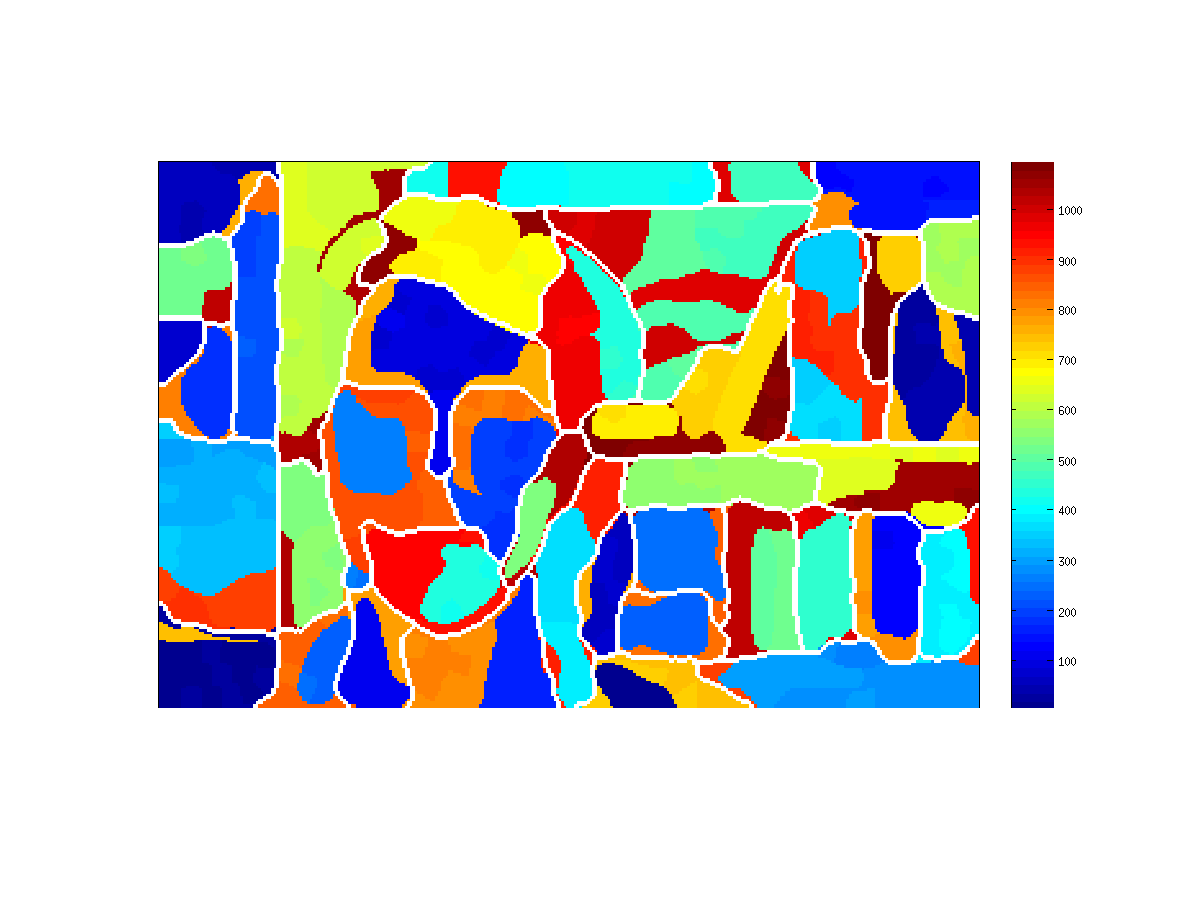
\includegraphics[width = \textwidth]{./img/su6_3_s.pdf}
			\label{fig:6_3_s_su}
		\end{subfigure}
		\begin{subfigure}[c]{0.195\textwidth}
			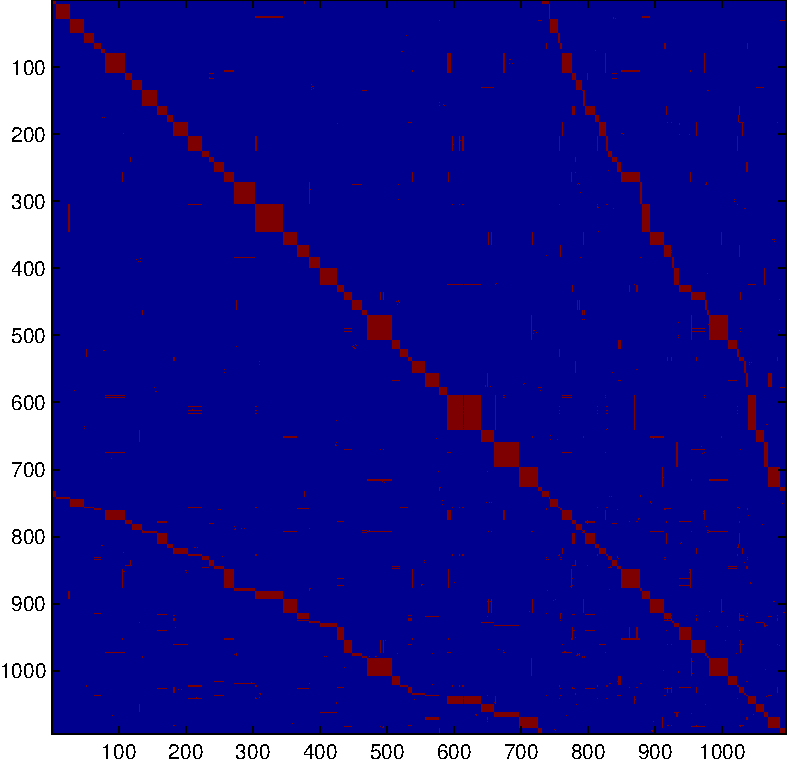
\includegraphics[width = \textwidth]{./img/adj6_3_s.pdf}
			\label{fig6_3_s_adj}
		\end{subfigure}
	\end{subfigure}

	\begin{subfigure}[c]{\textwidth}
		\centering
		\begin{subfigure}[c]{0.195\textwidth}
			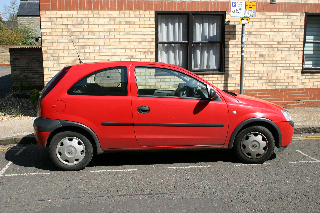
\includegraphics[width = \textwidth]{./img/7_8_s.png}
			\label{fig:7_8_s}

		\end{subfigure}
		\begin{subfigure}[c]{0.195\textwidth}
			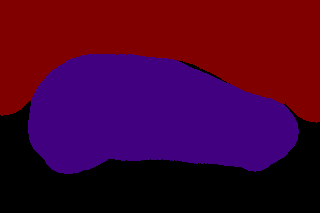
\includegraphics[width = \textwidth]{./img/7_8_s_GT.png}
			\label{fig:7_8_s_lab}
		\end{subfigure}
		\begin{subfigure}[c]{0.195\textwidth}
			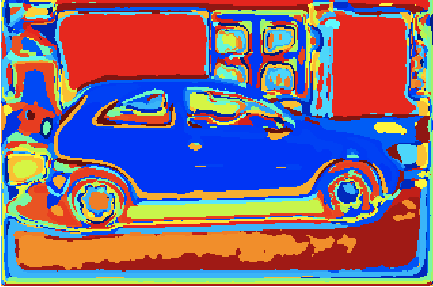
\includegraphics[width = \textwidth]{./img/7_8_s_map.png}
			\label{fig:7_8_s_map}
		\end{subfigure}
		\begin{subfigure}[]{0.195\textwidth}
			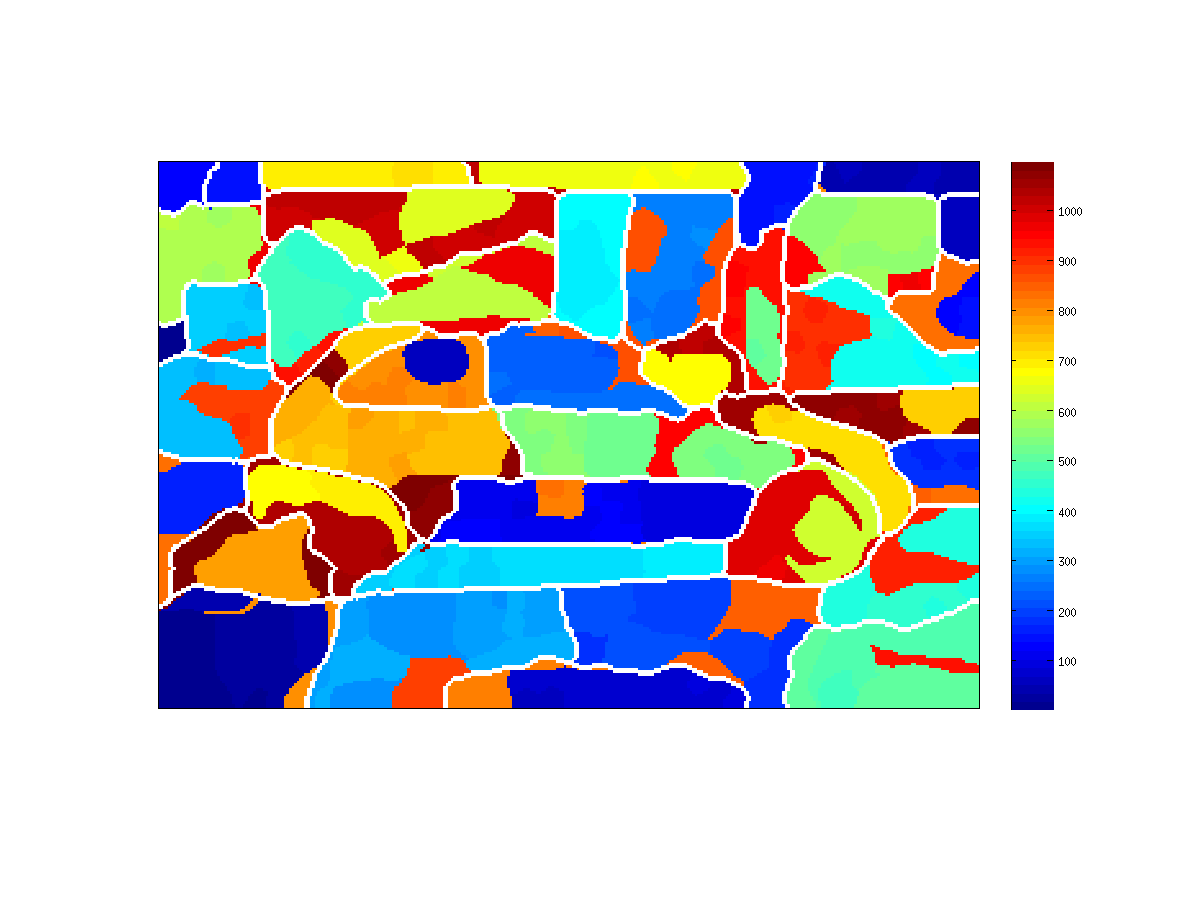
\includegraphics[width = \textwidth]{./img/su7_8_s.pdf}
			\label{fig:7_8_s_su}
		\end{subfigure}
		\begin{subfigure}[c]{0.195\textwidth}
			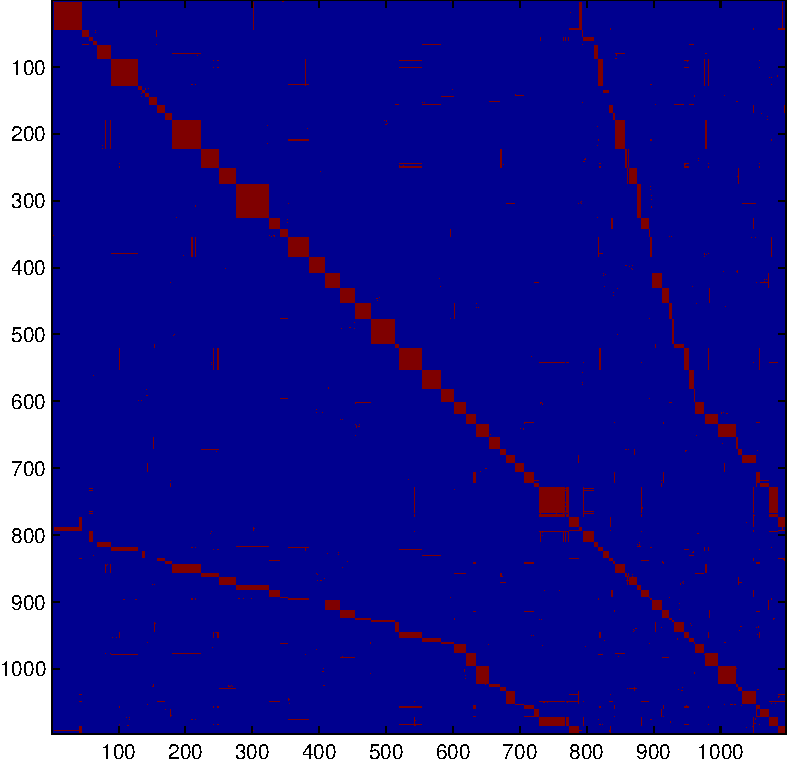
\includegraphics[width = \textwidth]{./img/adj7_8_s.pdf}
			\label{fig7_8_s_adj}
		\end{subfigure}
	\end{subfigure}

	
	\begin{subfigure}[t]{\textwidth}
		\centering
		\begin{subfigure}[t]{0.195\textwidth}
			\subcaption{original image}
		\end{subfigure}
		\begin{subfigure}[t]{0.195\textwidth}
			\subcaption{ground truth segmentation}
		\end{subfigure}
		\begin{subfigure}[t]{0.195\textwidth}
			\subcaption{visual words map}
		\end{subfigure}
		\begin{subfigure}[t]{0.195\textwidth}
			\subcaption{superpixel segmentation}
		\end{subfigure}
		\begin{subfigure}[t]{0.195\textwidth}
			\subcaption{superpixel adjacency matrix}
		\end{subfigure}
	\end{subfigure}

	\caption{}
\end{figure}
%------------------------------------------------------------------------------------------

\section{Conclusion}

%------------------------------------------------------------------------------------------
\section{Design of Upcoming Experiments}

%------------------------------------------------------------------------------------------
\section{Plan of Activities}

%------------------------------------------------------------------------------------------\bibliography{midway_report}
\bibliographystyle{plain}
\end{document}
